\setAuthor{Siim Ainsaar}
\setRound{lõppvoor}
\setYear{2012}
\setNumber{G 5}
\setDifficulty{6}
\setTopic{Kinemaatika}

\prob{Rehvid}
Et autorehvid kuluksid vähimal määral, tasub auto ehitada nii, et kurvis
pöörduksid esirattad eri nurga võrra. Leidke selles mõttes parim parema
esiratta pöördenurk $\beta$ paremkurvis, kus
vasaku esiratta oma on $\alpha$. Rataste vahekaugus on pikkupidi $a$ ja laiupidi
$b$ (vt joonist).
\begin{center}
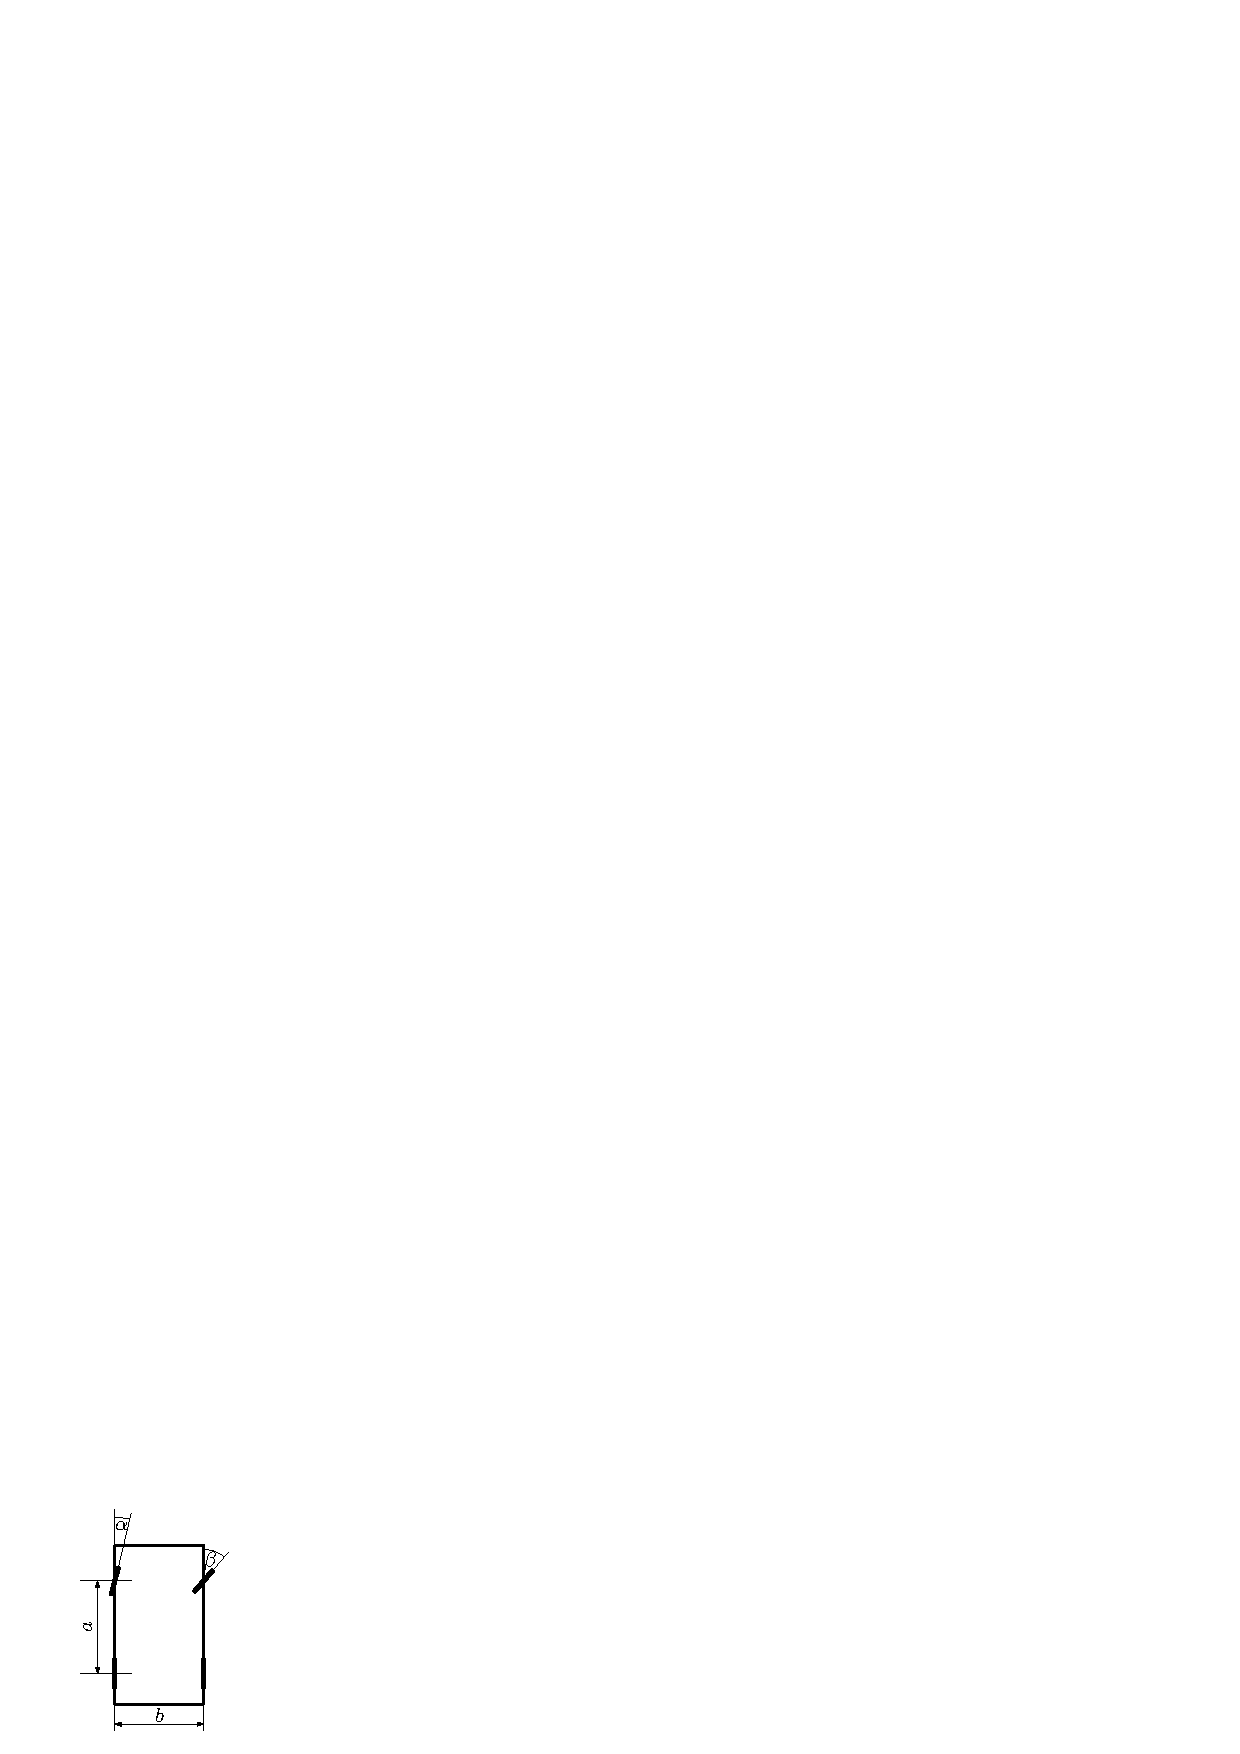
\includegraphics[width=0.3\linewidth]{2012-v3g-05-r_yl_joonis}%
\end{center}

\hint
Selleks, et autorehvid kuluksid vähimal määral, peavad rattad pöörama ühtse kehana. Kuna rattad ei libise, asub pöörlemiskese rataste teljel.

\solu
\begin{wrapfigure}{r}{0.4\textwidth}
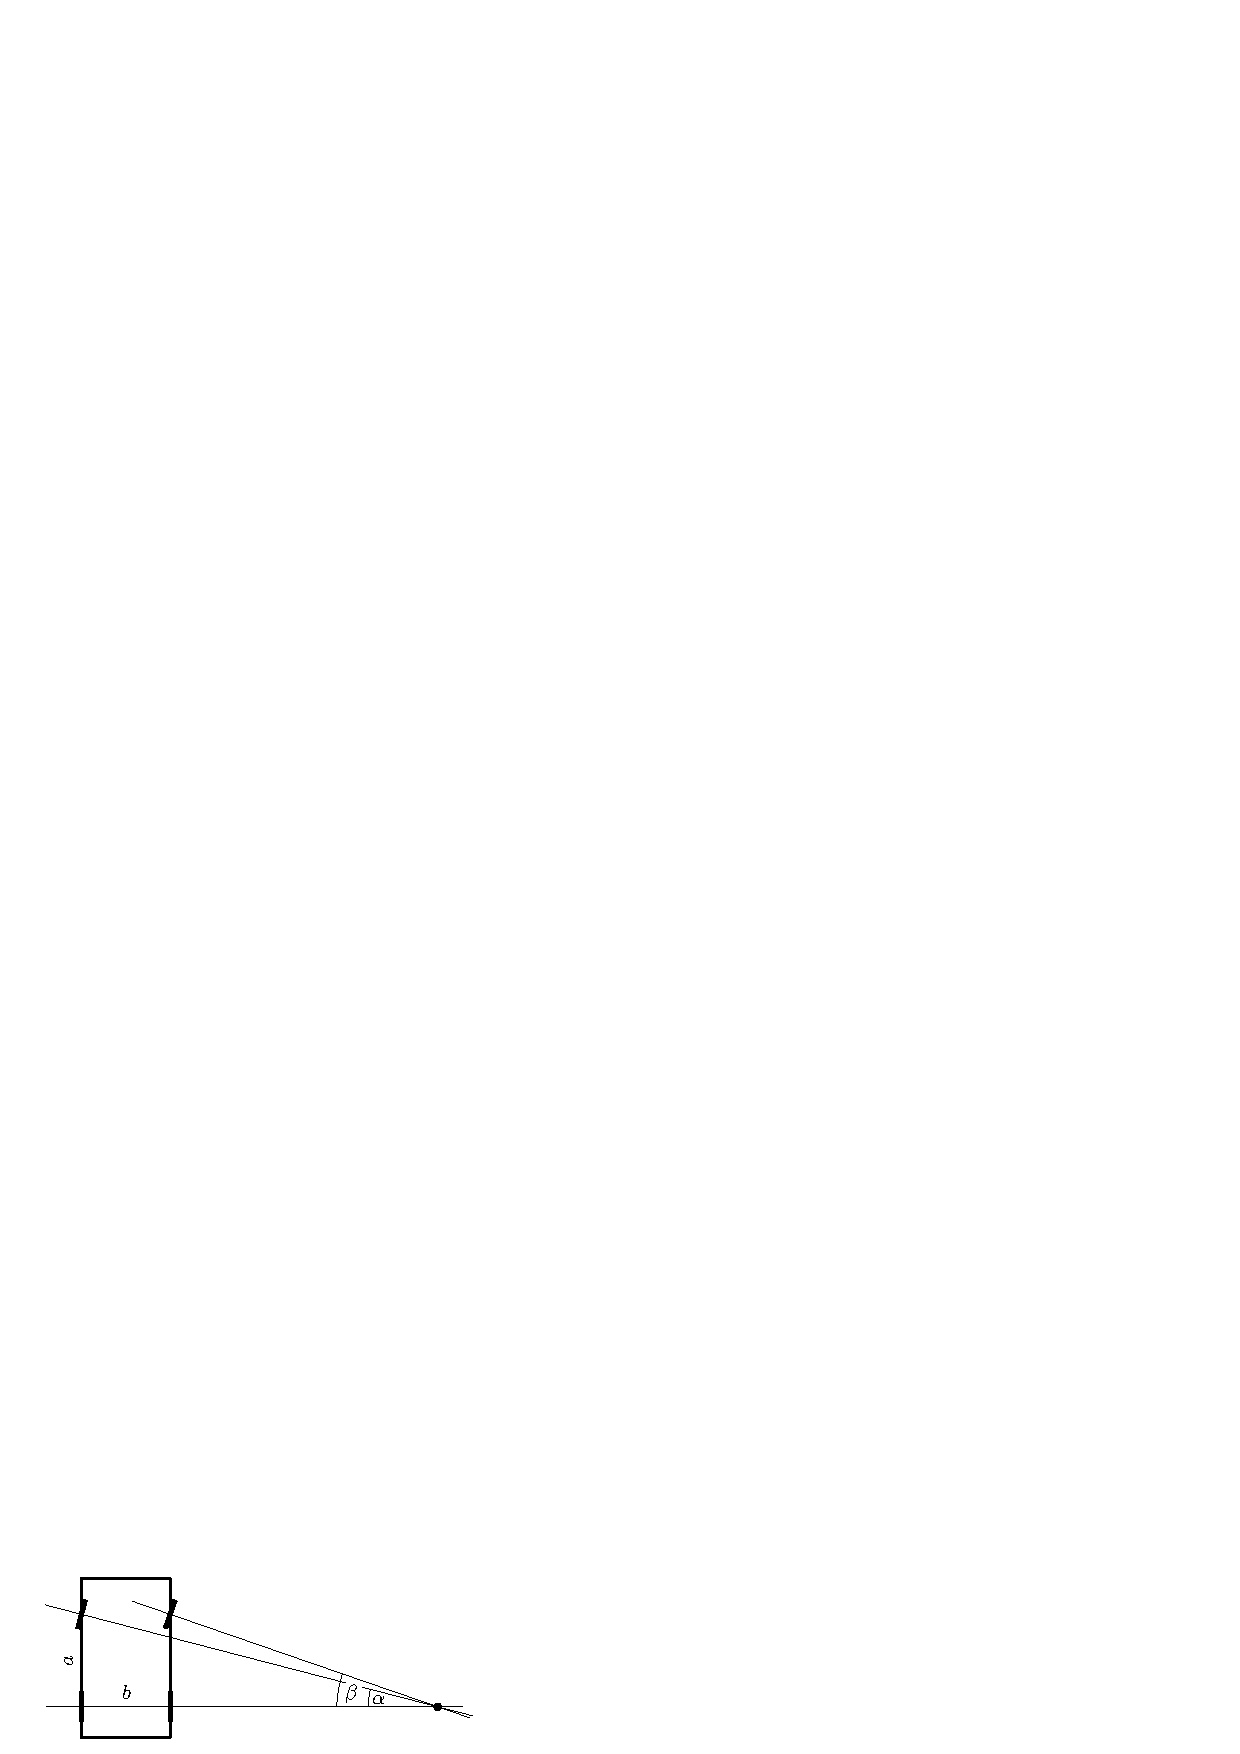
\includegraphics[width=\linewidth]{2012-v3g-05-r_joonis}
\end{wrapfigure}
Rattad tuleb pöörata suunda, mis ühtib nende liikumissuunaga. Ilmselt asub auto
pöörlemistelg tagarataste telgedega samal sirgel. Samas asub see optimaaljuhul
ka nii vasaku kui ka parema esiratta teljel. Seega otsitav nurk
\[
\beta =
\operatorname{arccot} \left( \frac{a \cot\alpha - b}{a} \right)
=
\operatorname{arccot} \left( \cot\alpha - \frac ba \right).
\]

\probeng{Tires}
For a car’s tires to wear as little as possible, the car should be built so that the front wheels would turn by a different angle on a curve. Find the best angle of rotation $\beta$ for the right front wheel on a right curve if the angle for the left front wheel is $\alpha$. The distance between the wheels longitudinally is $a$ and laterally is $b$ (see figure).
\begin{center}
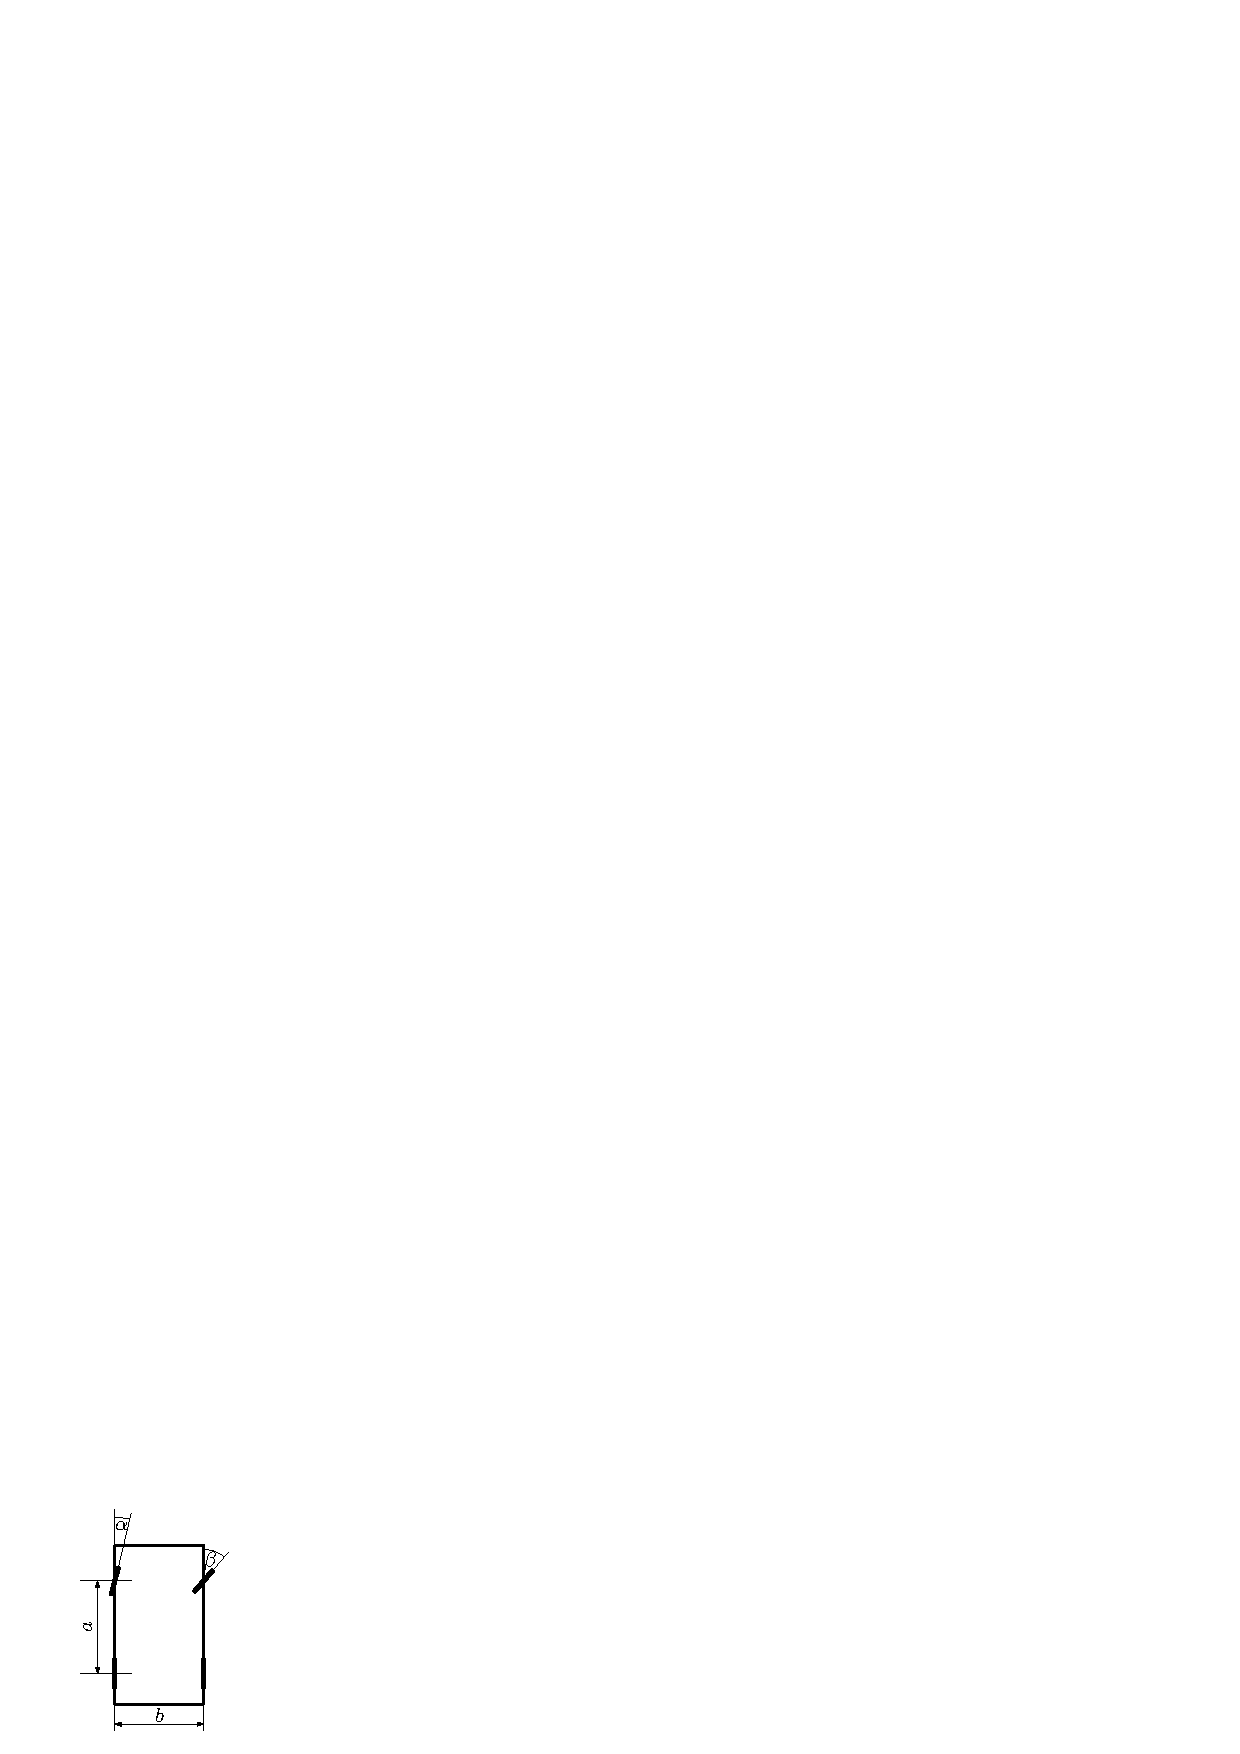
\includegraphics[width=0.3\linewidth]{2012-v3g-05-r_yl_joonis}%
\end{center}

\hinteng
For the car tires to wear as little as possible the wheels have turn as one body. Since the wheels do not slide the center of rotation is located on the axis of the wheels.

\solueng
\begin{wrapfigure}{r}{0.4\textwidth}
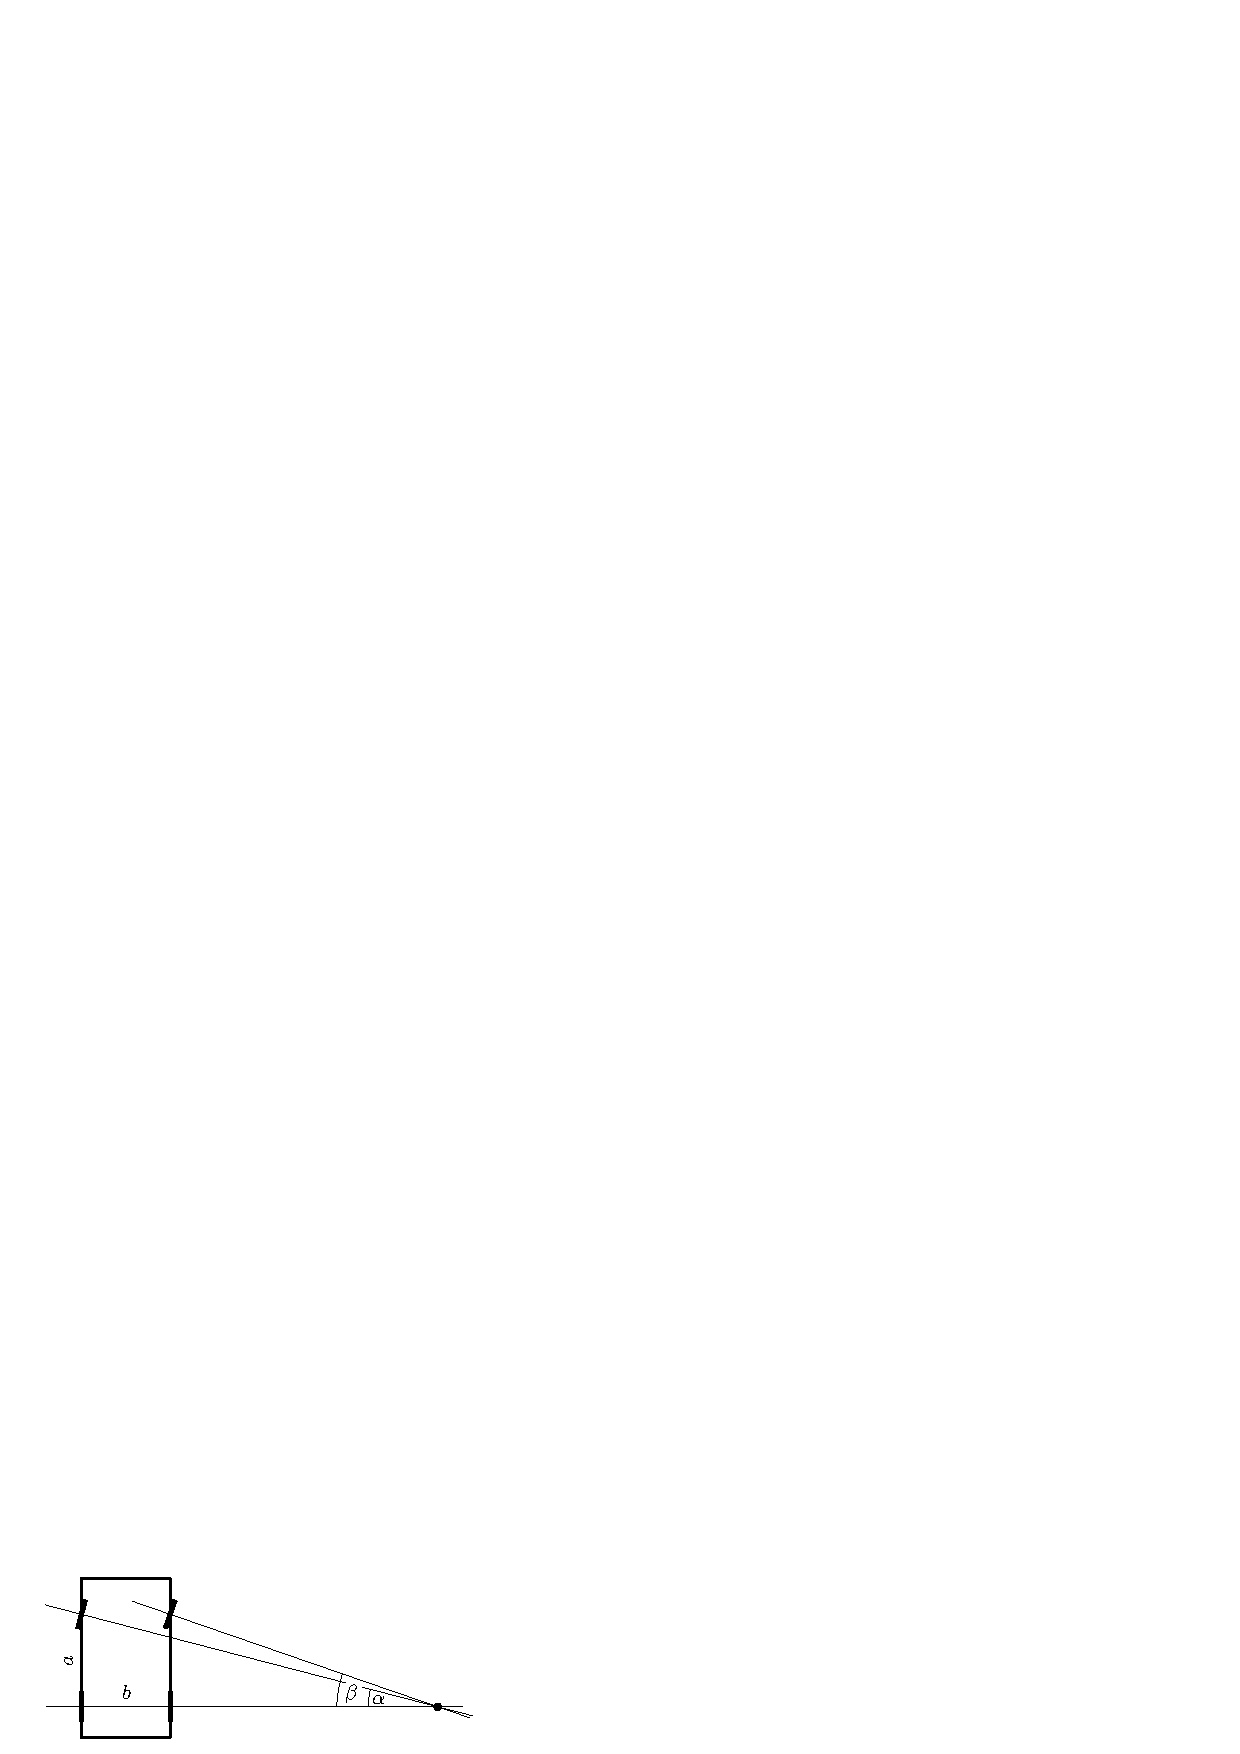
\includegraphics[width=\linewidth]{2012-v3g-05-r_joonis}
\end{wrapfigure}
The tires have to be turned to a direction that coincides with their movement direction. The car’s rotation axis is probably located on the same line as the axes of the rear wheels. On the other hand in the optimal case it would also be located on both the right and left front wheel’s axis. Therefore the desired angle
\[
\beta =
\operatorname{arccot} \left( \frac{a \cot\alpha - b}{a} \right)
=
\operatorname{arccot} \left( \cot\alpha - \frac ba \right).
\]
\probend